\documentclass[tikz,border=2pt]{standalone}

\usepackage{pgfplots}
\pgfplotsset{compat=1.18}

\begin{document}
	
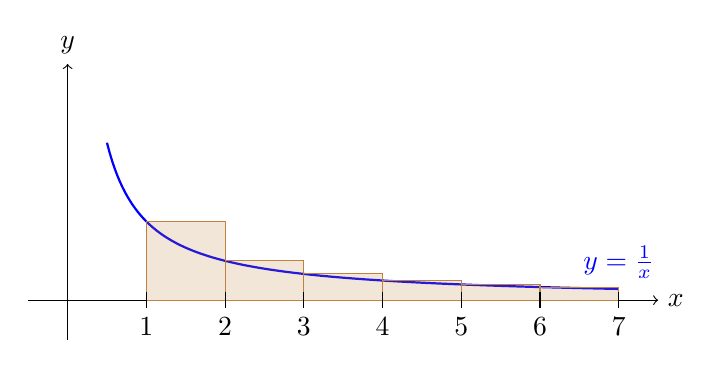
\begin{tikzpicture}
	% Draw the axes
	\draw[->] (-0.5,0) -- (7.5,0) node[right] {$x$};
	\draw[->] (0,-0.5) -- (0,3) node[above] {$y$};
	% Draw the function y=1/x
	\draw[blue, thick, domain=0.5:7, samples=200, variable=\x] plot ({\x},{1/\x}) node[above] {$y=\frac{1}{x}$};
	% Draw the rectangles
	\foreach \x in {1,...,6} {
		\draw[brown, fill=brown, fill opacity=0.2] ({\x},0) rectangle ({\x+1},{1/\x});
	}
	% Add the x-axis labels
	\foreach \x in {1,...,7} {
		\draw (\x,0.1) -- (\x,-0.1) node[below] {\x};
	}
\end{tikzpicture}
	
\end{document}